\chapter{Going further : A word about nanowires}
\label{Chap5}

While I was making tests with the NIS junctions and the plasma, Mathieu started to build a recipe for the barrier nanowires.
       
    \section{Clean room process}
        
        The main question we have to ask is, starting from the methods seen in Chapter \ref{Chap2}, how can we integrate the nanowires to realize a real measureable structure.
                
        \subsection{Observation and EBL}
        
        First of all, we receive the nanowires as they were made which means half-covered by Al and randomly dispatched upon the wafer's surface (Fig. \ref{NWfirst}). The goal is to realize NISIN structures with Cu leads as normal metal, InGaAs barriers as insulators and the nanowire as superconductor thanks to Al and induced superconductivity. First, we will try to realize only NIS, by cov ering one of the barriers with Al, to see if the process can work out. The first thing we have to do is to observe the chip to find some wire that seems good enough to be exploited, get their coordinates on the surface and design a pattern to draw with the EBL.
        
        \begin{figure}
            \centering
            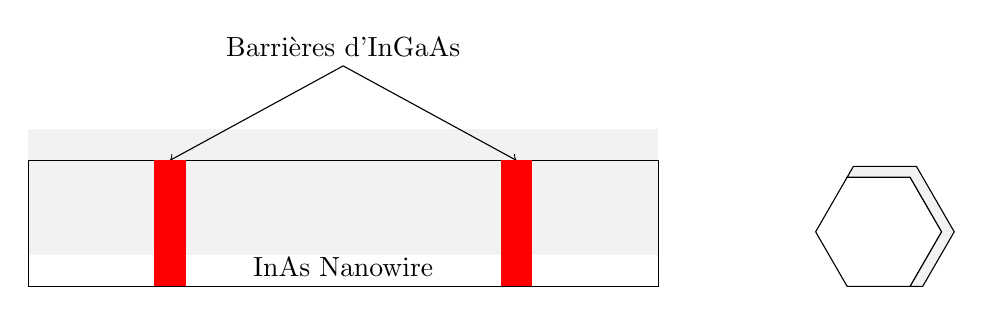
\begin{tikzpicture}[scale=0.8]
                \fill [color=gray!10] (0,0.5)--(10,0.5)--(10,2.5)--(0,2.5)--cycle;
                \draw (0,0)--(10,0)--(10,2)--(0,2)--cycle;
                \draw [<-] (2.25,2)--(5,3.5);
                \draw [<-] (7.75,2)--(5,3.5);
                \draw (5,3.5)node[above]{Barrières d'InGaAs};
                \draw (5,0.3) node{InAs Nanowire};
                \fill [color=red] (2,0)--(2.5,0)--(2.5,2)--(2,2)--cycle;
                \fill [color=red] (8,0)--(7.5,0)--(7.5,2)--(8,2)--cycle;
                \draw (13,0)--++(1,0)--++({cos(60)},{sin(60)})--++({-cos(60)},{sin(60)})--++(-1,0)--++({-cos(60)},{-sin(60)})--cycle;
                \filldraw [fill=gray!10, draw=black] (14,0)--++(0.2,0)--++({cos(60},{sin(60)})--++({-1.2*cos(60)},{1.2*sin(60)})--++(-1,0)--++({-0.2*cos(60)},{-0.2*sin(60)})--++(1,0)--++({cos(60},{-sin(60)})--cycle;  
            \end{tikzpicture}
            \caption{Nanowires as received from Copenhaguen}
            \label{NWfirst}
        \end{figure}
        
        
        \subsection{Aluminium Etching}
        
        Then, we do not want to have Aluminium over the whole nanowire, so we have to etch it which we will do chemically.
        
        \begin{figure}
            \centering
            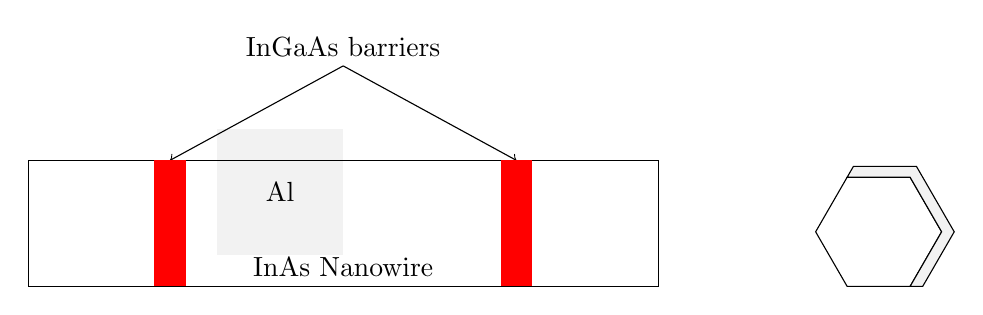
\begin{tikzpicture}[scale=0.8]
            
                \fill [color=gray!10] (3,0.5)--(5,0.5)--(5,2.5)--(3,2.5)--cycle;
                \draw (4,1.5)node{Al};
                \draw (0,0)--(10,0)--(10,2)--(0,2)--cycle;
                \draw [<-] (2.25,2)--(5,3.5);
                \draw [<-] (7.75,2)--(5,3.5);
                \draw (5,3.5)node[above]{InGaAs barriers};
                \draw (5,0.3) node{InAs Nanowire};
                \fill [color=red] (2,0)--(2.5,0)--(2.5,2)--(2,2)--cycle;
                \fill [color=red] (8,0)--(7.5,0)--(7.5,2)--(8,2)--cycle;
                
                \draw (13,0)--++(1,0)--++({cos(60)},{sin(60)})--++({-cos(60)},{sin(60)})--++(-1,0)--++({-cos(60)},{-sin(60)})--cycle;
                 \filldraw [fill=gray!10, draw=black] (14,0)--++(0.2,0)--++({cos(60},{sin(60)})--++({-1.2*cos(60)},{1.2*sin(60)})--++(-1,0)--++({-0.2*cos(60)},{-0.2*sin(60)})--++(1,0)--++({cos(60},{-sin(60)})--cycle;  
            \end{tikzpicture}
            \caption{Nanowires after Al etching}
        \end{figure}
        
        \subsection{Leads evaporation}
        
        Finally, we will evaporate the leads on the nanowire, with the evaporator.
               
                
            \begin{figure}
            \centering
            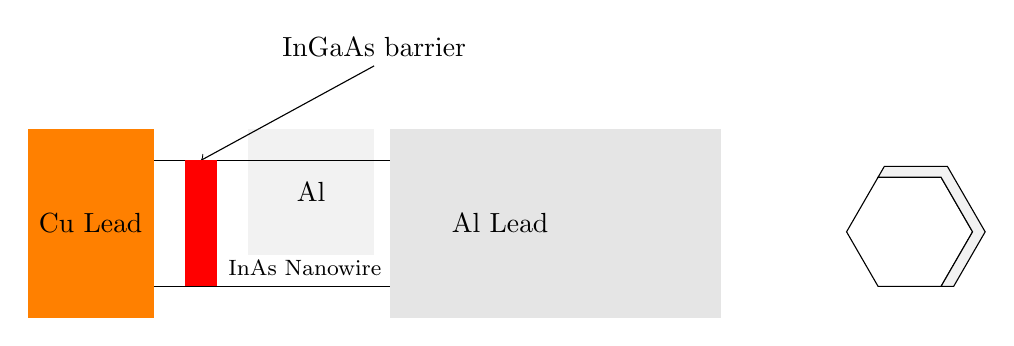
\begin{tikzpicture}[scale=0.8]
            
                \fill [color=gray!10] (3,0.5)--(5,0.5)--(5,2.5)--(3,2.5)--cycle;
                \draw (4,1.5)node{Al};
                \draw (0,0)--(10,0)--(10,2)--(0,2)--cycle;
                \draw [<-] (2.25,2)--(5,3.5);
                
                \fill [color=orange] (-0.5,-0.5)--(1.5,-0.5)--(1.5, 2.5)--(-0.5, 2.5)--cycle;
                \draw (0.5,1)node{Cu Lead};
                \fill [color=gray!20] (10.5,-0.5)--(5.25,-0.5)--(5.25,2.5)--(10.5,2.5)--cycle;
                \fill (7,1)node{Al Lead};
                \draw (5,3.5)node[above]{InGaAs barrier};
                \draw (3.9,0.3) node{{\footnotesize InAs Nanowire}};
                \fill [color=red] (2,0)--(2.5,0)--(2.5,2)--(2,2)--cycle;
                %\fill [color=red] (8,0)--(7.5,0)--(7.5,2)--(8,2)--cycle;
                \draw (13,0)--++(1,0)--++({cos(60)},{sin(60)})--++({-cos(60)},{sin(60)})--++(-1,0)--++({-cos(60)},{-sin(60)})--cycle;
                 \filldraw [fill=gray!10, draw=black] (14,0)--++(0.2,0)--++({cos(60},{sin(60)})--++({-1.2*cos(60)},{1.2*sin(60)})--++(-1,0)--++({-0.2*cos(60)},{-0.2*sin(60)})--++(1,0)--++({cos(60},{-sin(60)})--cycle;  
                 
                 
            \end{tikzpicture}
            \caption{Nanowires after evaporation}
            \end{figure}
        
